\section{Adding New Governing Equations and/or Bulk Rheologies}

There are four basic pieces to adding new physics in the form of a
governing equation:
\begin{enumerate}
\item Select the fields for the solution. This will control the form
  of the partial differential equation and the terms in the residuals
  and Jacobians.
\item Derive the point-wise functions for the residuals and
  Jacobians. Determine flags that will be used to indicate which terms
  to include.
\item Determine which parameters in the point-wise functions could
  vary in space as well as any state variables. We bundle all state variables
  and spatially varying parameters into a field called the auxiliary
  field. Each material has a separate auxiliary field.
\item Parameters that are spatially uniform are treated separately
  from the parameters in the auxliary field.
\end{enumerate}

The \object{Material} is responsible for the terms in the governing
equations associated with the domain (i.e., volume integrals in a 3D
domain and surface integrals in a 2D domain). A separate object
implements the bulk rheology for a specific governing
equation. Figure~\ref{fig:code:material} shows the objects used to
implement multiple rheologies for the elasticity equation and an
isotropic, linear elastic rheology for incompressible elasticity. The
\object{Elasticity} object describes the physics for the elasticity
equation, including the point-wise functions and flags for turning on
optional terms in the governing equation, and the
\object{RheologyElasticity} defines the interface for bulk elastic
rheologies.

\begin{figure}[htbp]
  \includegraphics[scale=0.8]{developer/figs/material_classdiagram}
  \caption{Class diagram for the implementation of governing equations
    and bulk rheologies. Each governing equation implementation
    inherits from the abstract \object{Material} class and bulk
    rheologies inherit from the abstract rheology class specific to
    that governing equation.}
  \label{fig:developer:material:class}
\end{figure}


\subsection{Python}

\begin{itemize}
\item Define solution subfields.

  \begin{itemize}
  \item All subfields in the solution field are
    \object{SolutionSubfield} objects (see
    \vref{fig:developer:solution:class}). PyLith already includes
    several solution subfields:
    \begin{description}
    \item[\object{SubfieldDisplacement}] Displacement vector field.
    \item[\object{SubfieldVelocity}] Velocity vector field.
    \item[\object{SubfieldLagrangeFault}] Lagrange multiplier field for
      fault constraints.
    \item[\object{SubfieldPressure}] Fluid pressure or mean stress scalar field.
    \item[\object{SubfieldTemperature}] Temperature scalar field.
    \end{description}
    %
  \item PyLith includes solution field containers with predefined
    subfields:
    \begin{description}
    \item[\object{SolnDisp}] Solution composed of a displacement field.
    \item[\object{SolnDispVel}] Solution composed of displacement and velocity fields.
    \item[\object{SolnDispPres}] Solution composed of displacement and
      mean stress (pressure) fields.
    \item[\object{SolnDispLagrange}] Solution composed of displacement
      and Lagrange multiplier fields.
    \item[\object{SolnDispPresLagrange}] Solution composed of
      displacement, mean stress (pressure), and Lagrange multiplier subfields.
    \item[\object{SolnDispVelLagrange}] Solution composed of
      displacement, velocity, and Lagrange multiplier subfields.
    \end{description}
  \end{itemize}
%
\item Define auxiliary subfields.

  The auxiliary subfields for a governing equation are defined as
  facilities in a Pyre Component. For example, the ones for
  \object{Elasticity} are in \object{AuxFieldsElasticity}. The order
  of the subfields is defined {\em not} by the order they are listed
  in the Pyre component, but by the order they are added to the
  auxiliary field in the C++ object. The auxiliary subfields bulk
  rheologies are defined in the same way.

  \important{A single auxiliary field will be created for each
    material; it contains the auxiliary subfields from both the
    governing equation and the bulk rheology}.

\item Flags to turn on/off terms in governing equation.

  For the elasticity equation, we sometimes do not include body forces
  or inertial terms in our simulations. Rather than implement these
  cases as separate materials, we simply include flags in the material
  to turn these terms on/off. The flags are implemented as Pyre
  properties in our material component.
\end{itemize}

\begin{figure}[htbp]
  \includegraphics[scale=0.8]{developer/figs/solution_classdiagram}
  \caption{Class diagram for the solution field, solution subfields,
    and pre-defined containers of solution subfields.}
  \label{fig:developer:solution:class}
\end{figure}

\subsection{C++}

\begin{itemize}
\item Define auxiliary subfields.

  We build the auxiliary field using classes derived from
  \object{pylith::feassemble::AuxiliaryFactory}. The method
  corresponding to each subfield specifies the name of the subfield,
  its components, and scale for nondimensionalizing. We generally
  create a single auxiliary factory object for each governing equation
  but not each bulk constitutive model, because constitutive models
  for the same governing equation often have many of the same
  subfields. For example, most of our bulk constitutive models for the
  elasticity contain density, bulk modulus, and shear modulus
  auxiliary subfields.

  \important{Within the concrete implementation of the material and
    bulk rheology objects, we add the subfields to the auxiliary
    field. The order in which they are added determines the order they
    will be in the auxiliary field. You will need to use know this
    order when you implement the point-wise functions. See
    Figure~\vref{fig:developer:material:auxiliary:field} for more
    information on the layout of the auxiliary field.}

\item Implement the point-wise functions.

  The point-wise functions for the residuals, Jacobians, and
  projections follow nearly identical interfaces. Note that within
  PyLith, we use PylithInt, PylithReal, and PylithScalar instead of
  PetscInt, PetscReal, and PetscScalar.

\item Set the point-wise functions.

  We set the point-wise functions for the RHS and LHS residuals and
  Jacobians, taking into consideration which optional terms of the
  governing equation have been selected by the user.

\end{itemize}

\begin{figure}[htbp]
  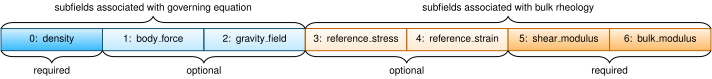
\includegraphics[scale=0.8]{developer/figs/material_auxiliarylayout}
  \caption{Layout of material auxiliary subfields. The subfields
    include those for both the governing equation and the bulk
    rheology. The required subfields are at the ends with the optional
    fields in the middle. This allows the same point-wise functions to
    be used for some cases with and without the optional subfields.}
  \label{fig:developer:material:auxiliary:subfield}
\end{figure}

\subsection{C++ Unit Tests}

The C++ unit tests focus on testing all methods of a C++ object. For
materials, this includes the accessors, factory methods, and setting
the residual and Jacobian point-wise function (kernels).

\subsection{C++ MMS Tests}

We use the Method of Manufactured Solutions to test the implementation
of the material. These tests check the representation of the solution
in the finite-element space, the residual, and the Jacobian. The
\object{UserFunctionDB} spatial database allows us to populate the
auxiliary field and solution using anlytical functions.

We check the residual by verifying that the residual computed for a
known solution is below some tolerance, $\epsilon$,
\begin{equation}
  || F(\vec{s}) - G(\vec{s}) || \le \epsilon,
\end{equation}
where $F(\vec{s})$ is the LHS residual and $G(\vec{s})$ is the RHS
residual.

We test the Jacobian using a Taylor series expansion and brute force
through finite differences. In the Talor series test, we verify that
\begin{equation}
  || F(\vec{s} + \epsilon \vec{v}) - F(\vec{s}) - \epsilon J \vec{v} || < \epsilon^2,
\end{equation}
where $\vec{v}$ is a perturbation in the soluton and $J$ is the
Jacobian matrix.  In the finit-difference test, we verify that each
value in the Jacobian matrix matches the value computed using
finite-differences to within some tolerance.


\todo{brad}{Update figure for MMS test.}
\begin{figure}[htbp]
  \includegraphics[scale=0.8]{developer/figs/testmaterial_classdiagram}
  \caption{Class diagram for testing the
    \object{IsotropicLinearElasticityPlaneStrain} material with a
    solution generated using the Method of Manufactured
    Solutions. \object{TestIsotropicLinearElasticityPlaneStrain\_UniformStrain}
    contains the parameters and generated solution and the subclasses
    include various discretizations. All of the test data is held in
    the \object{TestIsotropicLinearElasticityPlaneStrain\_Data}
    object.}
  \label{fig:developer:test:material:class}
\end{figure}


\subsection{Python Unit Tests}

With the Python implementation focused on gathering the user configuration of a simulation, there is
minimal functionality we can test at the Python level. Consequently, the Python unit tests are generally
limited to testing the SWIG interface, which involves creating the C++ object and insuring the Pyre
properties and facilities and any other information is passed to the C++ object.

\subsection{Full-Scale Tests}

\todo{brad}{Add figure for full-scale test}


% End of file
